%\section{Descipción de casos de uso}
\noindent
En esta sección presentamos los módulos que componen a la aplicación ESCOMobile así como al sistema web
complementario ESCOMobile Bolsa, así como los casos de uso que forman parte a cada uno de estos módulos
que en conjunto hacen un único sistema.   

\noindent
\newline
Así, los módulos de los cuales ESCOMobile se compone son los siguientes: 
	\begin{itemize}
        \item Acceso.
        \item Mapa.
        \item Alumno.
        \item AlumnoBolsa.
        \item AlumnoProfesor.
        \item Profesor.
        \item Citas.
        \item BolsaWeb.
	\end{itemize}

\noindent
A continuación se explican de forma individual los módulos mencionados y los casos de uso que los conforman. 


%%%%%%%%%%%%%%%%%%%%%%%%%%%%%%%%%%%%%%%%%%%%%%%%%%%%%%%%%%%%%%%%%%%%%%%%%%%%%%%%%%%%%%%%%%%%%%%%%%%%%%%%%%%%%%%
%												MÓDULO DE ACCESO
%%%%%%%%%%%%%%%%%%%%%%%%%%%%%%%%%%%%%%%%%%%%%%%%%%%%%%%%%%%%%%%%%%%%%%%%%%%%%%%%%%%%%%%%%%%%%%%%%%%%%%%%%%%%%%%


\section{Módulo de Acceso}

\noindent
Este módulo presenta la introducción de la app al usuario, es aquí donde se realiza el registro y el acceso 
a la app y a su contenido. Cuenta con con un total de 6 casos de uso que se enlistan debajo.

\begin{requisitos}{EM-Acceso-CU1}
	\RFitem{Nombre}{Registrar nuevo usuario.}
	\RFitem{Actores}{Alumno, Profesor.}
\end{requisitos}

\begin{requisitos}{EM-Acceso-CU2}
	\RFitem{Nombre}{Iniciar sesión.}
	\RFitem{Actores}{Alumno, Profesor.}
\end{requisitos}

\begin{requisitos}{EM-Acceso-CU3}
	\RFitem{Nombre}{Recuperar contraseña.}
	\RFitem{Actores}{Alumno, Profesor.}
\end{requisitos}

\begin{requisitos}{EM-Acceso-CU4}
	\RFitem{Nombre}{Cerrar Sesión.}
	\RFitem{Actores}{Alumno, Profesor.}
\end{requisitos}

\begin{requisitos}{EM-Acceso-CU5}
	\RFitem{Nombre}{Eliminar cuenta}
	\RFitem{Actores}{Alumno, Profesor.}
\end{requisitos}

\begin{requisitos}{EM-Acceso-CU6}
	\RFitem{Nombre}{Consultar Información de ESCOMobile.}
	\RFitem{Actores}{Alumno, Profesor, Invitado.}
\end{requisitos}

\noindent
A continuación se presenta el diagrama de casos de uso referente a este módulo, en donde se pueden apreciar
los casos dde uso anteriormente presentados y su interacción con los actores.

\pagebreak
\begin{figure}[htbp!]
	\centering
	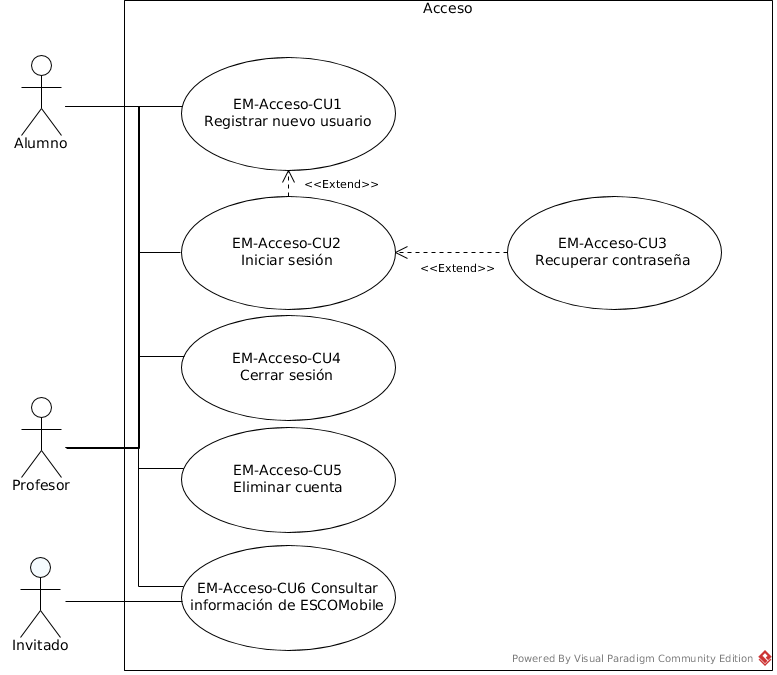
\includegraphics[width=0.8\textwidth]{images/casos/acceso}
	\caption{Diagrama de casos de uso ESCOMobile: Acceso.}
\end{figure}


%%%%%%%%%%%%%%%%%%%%%%%%%%%%%%%%%%%%%%%%%%%%%%%%%%%%%%%%%%%%%%%%%%%%%%%%%%%%%%%%%%%%%%%%%%%%%%%%%%%%%%%%%%%%%%%
%												MÓDULO DE MAPA
%%%%%%%%%%%%%%%%%%%%%%%%%%%%%%%%%%%%%%%%%%%%%%%%%%%%%%%%%%%%%%%%%%%%%%%%%%%%%%%%%%%%%%%%%%%%%%%%%%%%%%%%%%%%%%%


\section{Módulo de Mapa}

\noindent
Este módulo nos muestra la ventana principal de la app móvil ESCOMobile, el mapa de ESCOM, y
la primera gran acción que se presenta en él, la búsqueda de profesres, salones, cubículos o academias. 
Se compone únicamente de dos casos de uso, que son:

\begin{requisitos}{EM-Mapa-CU1}
	\RFitem{Nombre}{Consulta Mapa de ESCOM.}
	\RFitem{Actores}{Alumno, Profesor, Invitado.}
\end{requisitos}

\begin{requisitos}{EM-Mapa-CU2}
	\RFitem{Nombre}{Realizar búsqueda sobre el mapa.}
	\RFitem{Actores}{Alumno, Profesor, Invitado.}
\end{requisitos}

\noindent
El diagrama de casos de uso que modela los dos anteriores se presenta aquí debajo.

\pagebreak
\begin{figure}[htbp!]
	\centering
	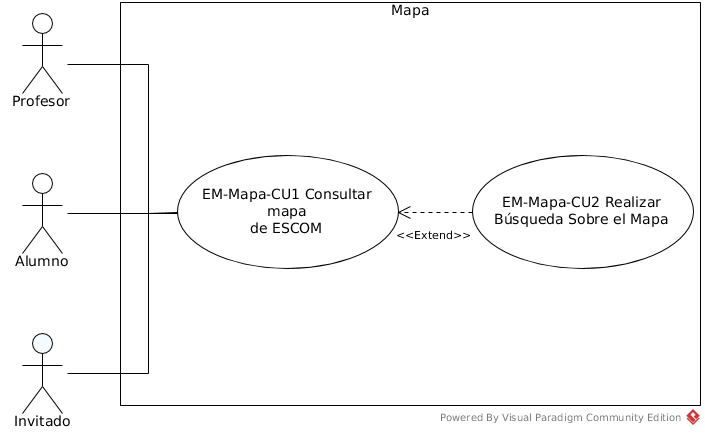
\includegraphics[width=0.8\textwidth]{images/casos/mapa}
	\caption{Diagrama de casos de uso ESCOMobile: Mapa.}
\end{figure}


%%%%%%%%%%%%%%%%%%%%%%%%%%%%%%%%%%%%%%%%%%%%%%%%%%%%%%%%%%%%%%%%%%%%%%%%%%%%%%%%%%%%%%%%%%%%%%%%%%%%%%%%%%%%%%%
%												MÓDULO DE ALUMNO
%%%%%%%%%%%%%%%%%%%%%%%%%%%%%%%%%%%%%%%%%%%%%%%%%%%%%%%%%%%%%%%%%%%%%%%%%%%%%%%%%%%%%%%%%%%%%%%%%%%%%%%%%%%%%%%


\section{Módulo de Alumno}

\noindent
Este módulo nos presenta la posibilidad que tiene un alumno de la ESCOM de controlar su información
en la aplicación, esto es, consulta y actualizar ésta cuando sea necesario. El módulo consta de dos 
casos de uso dedicados al alumno y su información, éstos se mencionan a continuación:

\begin{requisitos}{EM-Alumno-CU1}
	\RFitem{Nombre}{Consultar Perfil del Alumno.}
	\RFitem{Actores}{Alumno.}
\end{requisitos}

\begin{requisitos}{EM-Alumno-CU1.1}
	\RFitem{Nombre}{Modificar Información.}
	\RFitem{Actores}{Alumno.}
\end{requisitos}

\noindent
Así bien, ahora se muestra el diagrama que describe lo antes mencionado. 

\pagebreak
\begin{figure}[htbp!]
	\centering
	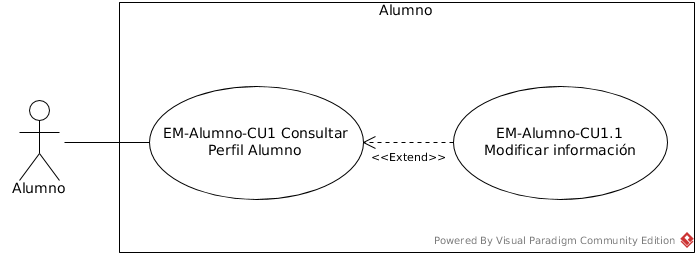
\includegraphics[width=0.8\textwidth]{images/casos/alumno}
	\caption{Diagrama de casos de uso ESCOMobile: Alumno.}
\end{figure}


%%%%%%%%%%%%%%%%%%%%%%%%%%%%%%%%%%%%%%%%%%%%%%%%%%%%%%%%%%%%%%%%%%%%%%%%%%%%%%%%%%%%%%%%%%%%%%%%%%%%%%%%%%%%%%%
%											MÓDULO DE ALUMNO BOLSA
%%%%%%%%%%%%%%%%%%%%%%%%%%%%%%%%%%%%%%%%%%%%%%%%%%%%%%%%%%%%%%%%%%%%%%%%%%%%%%%%%%%%%%%%%%%%%%%%%%%%%%%%%%%%%%%


\section{Módulo de AlumnoBolsa}

\noindent
Este módulo nos permite conocer las ofertas de trabajo disponibles para los alumnos o egresados de la ESCOM
por medio de la consulta de la Bolsa de trabajo de ESCOM, misma que se adapta a ESCOMobile como un módulo más, 
el módulo de ESCOMobile Bolsa, en donde se pueden, entre otras cosas registar empresas y ofertas de trabajo
dadas por las mismas para los alumos de la Superior de Cómputo. 
El módulo presente, para la consulta de ofertas de trabajo es móvil y cuenta con dos casos de uso que se
enlistan debajo.

\begin{requisitos}{EM-AlumnoBolsa-CU1}
	\RFitem{Nombre}{Consultar Bolsa de Trabajo.}
	\RFitem{Actores}{Alumno, Profesor.}
\end{requisitos}

\begin{requisitos}{EM-AlumnBolsa-CU1.1}
	\RFitem{Nombre}{Consultar Oferta de Trabajo.}
	\RFitem{Actores}{Alumno, Profesor.}
\end{requisitos}

\noindent
Se muestra también su correspondiente diagrama, que contiene los casos de uso, los actores que intervienen
y las relaciones existentes entre los anteriores y los caosos. 

\begin{figure}[htbp!]
	\centering
	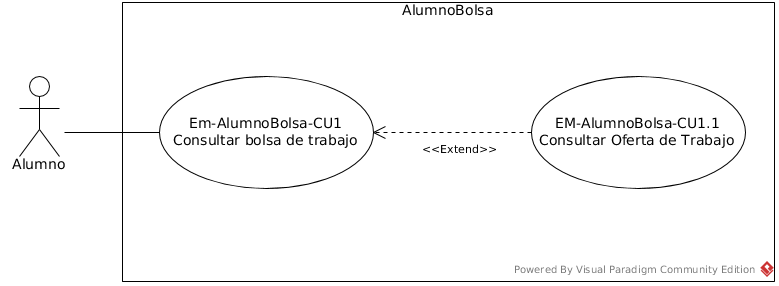
\includegraphics[width=0.8\textwidth]{images/casos/alumnoBolsa}
	\caption{Diagrama de casos de uso ESCOMobile: AlumnoBolsa.}
\end{figure}

\newpage


%%%%%%%%%%%%%%%%%%%%%%%%%%%%%%%%%%%%%%%%%%%%%%%%%%%%%%%%%%%%%%%%%%%%%%%%%%%%%%%%%%%%%%%%%%%%%%%%%%%%%%%%%%%%%%%
%											MÓDULO DE ALUMNOPROFESOR
%%%%%%%%%%%%%%%%%%%%%%%%%%%%%%%%%%%%%%%%%%%%%%%%%%%%%%%%%%%%%%%%%%%%%%%%%%%%%%%%%%%%%%%%%%%%%%%%%%%%%%%%%%%%%%%


\section{Módulo de AlumnoProfesor}

\noindent
Este módulo se centra en la interacción que alumnos y profesores de ESCOM logran gracias a la aplicación.
Es aquí donde se establecen los puntos que los usuarios tienen para realizar búsquedas de profesores para
llevar a cabo tareas específicas, como lo son la consulta de la información básica de algún profesor de
interés, así como el horario, estadísticas o los comentarios asociados a los antes mencionados. Se establecen
de igual manera acciones que nos redirigen a otros módulos de la app, como lo son el ubicar al profesor en el
mapa o solicitar una cita. 
El módulo se compone de ocho casos de uso, mismos que ahora se describen.

\begin{requisitos}{EM-AlumnoProfesor-CU1}
	\RFitem{Nombre}{Buscar Profesor de ESCOM.}
	\RFitem{Actores}{Alumno, Profesor.}
\end{requisitos}

\begin{requisitos}{EM-AlumnoProfesor-CU1.1}
	\RFitem{Nombre}{Consultar Perfil de Profesor.}
	\RFitem{Actores}{Alumno.}
\end{requisitos}

\begin{requisitos}{EM-AlumnoProfesor-CU1.1.1}
	\RFitem{Nombre}{Consultar Horario del Profesor.}
	\RFitem{Actores}{Alumno, Profesor.}
\end{requisitos}

\begin{requisitos}{EM-AlumnoProfesor-CU1.1.2}
	\RFitem{Nombre}{Calificar Desempeño de Profesor.}
	\RFitem{Actores}{Alumno.}
\end{requisitos}

\begin{requisitos}{EM-AlumnoBolsa-CU1.1.3}
	\RFitem{Nombre}{Consultar Estadísticas del Profesor.}
	\RFitem{Actores}{Alumno, Profesor.}
\end{requisitos}

\begin{requisitos}{EM-AlumnoProfesor-CU1.1.3.1}
	\RFitem{Nombre}{Consultar Comentarios del Profesor.}
	\RFitem{Actores}{Alumno, Profesor.}
\end{requisitos}

\begin{requisitos}{EM-AlumnoProfesor-CU1.1.4}
	\RFitem{Nombre}{Ubicar a Profesor en el Mapa.}
	\RFitem{Actores}{Alumno, Profesor.}
\end{requisitos}

\begin{requisitos}{EM-AlumnoProfesor-CU1.1.5}
	\RFitem{Nombre}{Solicitar Cita con Profesor.}
	\RFitem{Actores}{Alumno.}
\end{requisitos}

\noindent
Debajo se ecuentra el diagrama de casos de uso, donde se observa la interacción que hay
entre los casos de uso y los actores presentes.

\pagebreak
\begin{figure}[htbp!]
	\centering
	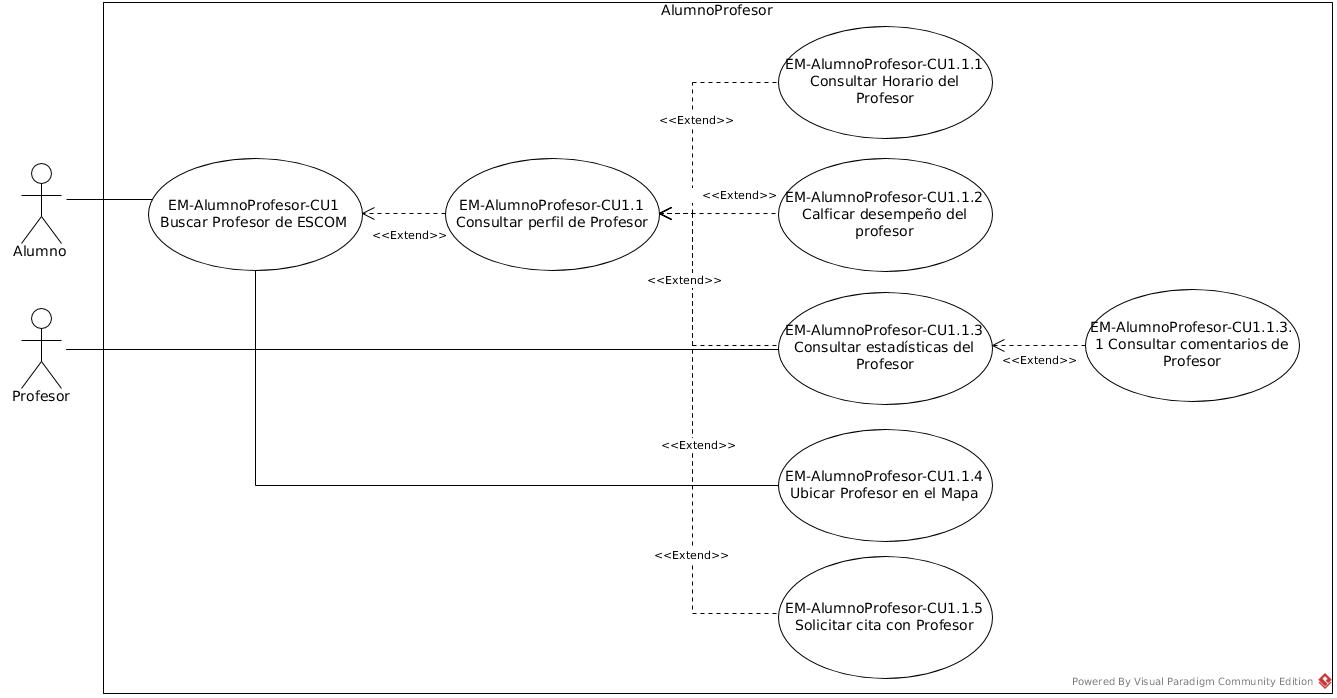
\includegraphics[width=1\textwidth]{images/casos/alumnoProfesor}
	\caption{Diagrama de casos de uso ESCOMobile: AlumnoProfesor.}
\end{figure}


%%%%%%%%%%%%%%%%%%%%%%%%%%%%%%%%%%%%%%%%%%%%%%%%%%%%%%%%%%%%%%%%%%%%%%%%%%%%%%%%%%%%%%%%%%%%%%%%%%%%%%%%%%%%%%%
%												MÓDULO DE PROFESOR
%%%%%%%%%%%%%%%%%%%%%%%%%%%%%%%%%%%%%%%%%%%%%%%%%%%%%%%%%%%%%%%%%%%%%%%%%%%%%%%%%%%%%%%%%%%%%%%%%%%%%%%%%%%%%%%


\section{Módulo de Profesor}

\noindent
Este módulo se enfoca en los profesores de la ESCOM y las acciones que pueden realizar con el sistema, así
como el cuidado de su información disponible para consulta dentro del mismo. Las acciones disponibles son la
consulta de su perfíl propio, horario, estadísticas y comentarios asignados, así como perfiles de otros profesores.
El módulo se compone pos los siguientes 6 casos de uso.

\begin{requisitos}{EM-Profesor-CU1}
	\RFitem{Nombre}{Consultar Perfil Propio.}
	\RFitem{Actores}{Profesor.}
\end{requisitos}

\begin{requisitos}{EM-Profesor-CU1.1}
	\RFitem{Nombre}{Consultar Horario Propio.}
	\RFitem{Actores}{Profesor.}
\end{requisitos}

\begin{requisitos}{EM-Profesor-CU1.2}
	\RFitem{Nombre}{Consultar Estadísticas Asignadas.}
	\RFitem{Actores}{Profesor.}
\end{requisitos}

\begin{requisitos}{EM-Profesor-CU1.2.1}
	\RFitem{Nombre}{Consultar Comentarios Asignados.}
	\RFitem{Actores}{Profesor.}
\end{requisitos}

\begin{requisitos}{EM-Profesor-CU1.3}
	\RFitem{Nombre}{Modificar Perfil del Profesor.}
	\RFitem{Actores}{Profesor.}
\end{requisitos}

\begin{requisitos}{EM-Profesor-CU2}
	\RFitem{Nombre}{Consultar Perfil de Otro Profesor.}
	\RFitem{Actores}{Profesor.}
\end{requisitos}

\noindent
A continuación se muestra la distribución de los casos de uso del módulo de Profesor.

\begin{figure}[htbp!]
	\centering
	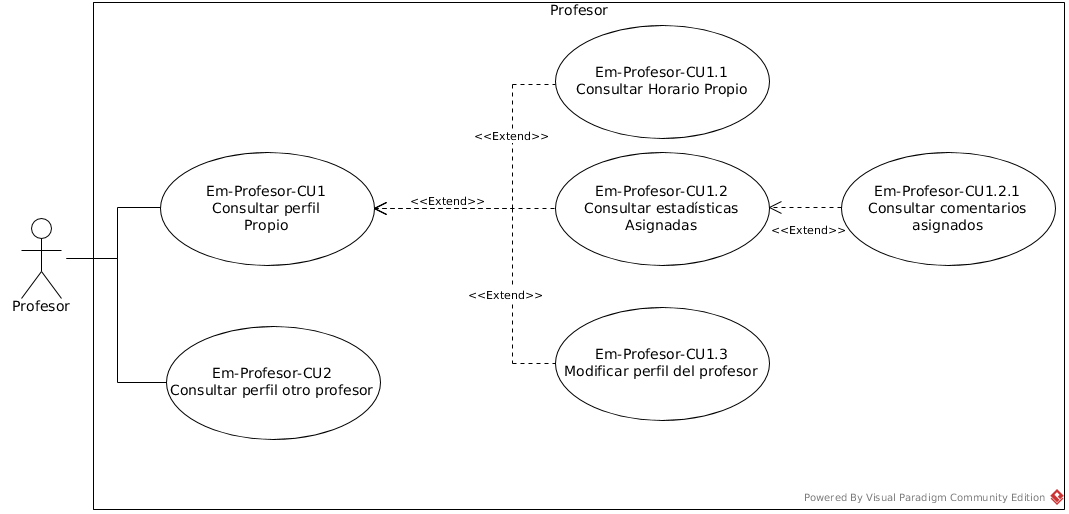
\includegraphics[width=1\textwidth]{images/casos/profesor}
	\caption{Diagrama de casos de uso ESCOMobile: Profesor.}
\end{figure}


%%%%%%%%%%%%%%%%%%%%%%%%%%%%%%%%%%%%%%%%%%%%%%%%%%%%%%%%%%%%%%%%%%%%%%%%%%%%%%%%%%%%%%%%%%%%%%%%%%%%%%%%%%%%%%%
%												MÓDULO DE CITAS
%%%%%%%%%%%%%%%%%%%%%%%%%%%%%%%%%%%%%%%%%%%%%%%%%%%%%%%%%%%%%%%%%%%%%%%%%%%%%%%%%%%%%%%%%%%%%%%%%%%%%%%%%%%%%%%


\section{Módulo de Citas}

\noindent
En este módulo se establecen las características de las citas entre alumnos y profesores de la ESCOM
y cómo éstas se llevan a cabo. Es aquí en donde, se definen los tipos de citas, la manera en que se observan
y se solicitan. En el presente módulo se compone de 9 casos de uso que se muestran debajo. 

\begin{requisitos}{EM-Citas-CU1}
	\RFitem{Nombre}{Consultar Citas agendadas.}
	\RFitem{Actores}{Alumno, Profesor.}
\end{requisitos}

\begin{requisitos}{EM-Citas-CU1.1}
	\RFitem{Nombre}{Cancelar Cita Asignada.}
	\RFitem{Actores}{Alumno, Profesor.}
\end{requisitos}

\begin{requisitos}{EM-Citas-CU1.2}
	\RFitem{Nombre}{Consultar Citas por Confirmar.}
	\RFitem{Actores}{Alumno, Profesor.}
\end{requisitos}

\begin{requisitos}{EM-Citas-CU1.2.1}
	\RFitem{Nombre}{Aceptar Cita por Confirmar.}
	\RFitem{Actores}{Profesor.}
\end{requisitos}

\begin{requisitos}{EM-Citas-CU1.2.2}
	\RFitem{Nombre}{Cancelar Cita por Confirmar.}
	\RFitem{Actores}{Alumno, Profesor.}
\end{requisitos}

\begin{requisitos}{EM-Citas-CU1.3}
	\RFitem{Nombre}{Consultar Citas Pasadas.}
	\RFitem{Actores}{Alumno, Profesor.}
\end{requisitos}

\begin{requisitos}{EM-Citas-CU1.3.1}
	\RFitem{Nombre}{Eliminar Citas Pasadas.}
	\RFitem{Actores}{Alumno, Profesor.}
\end{requisitos}

\begin{requisitos}{EM-Citas-CU2}
	\RFitem{Nombre}{Agendar una Cita.}
	\RFitem{Actores}{Alumno.}
\end{requisitos}

\begin{requisitos}{EM-Citas-CU2.1}
	\RFitem{Nombre}{Seleccionar Profesor para Cita.}
	\RFitem{Actores}{Alumno.}
\end{requisitos}

\noindent
En el siguiente diagrama de casos de uso se muestran los casos que componen al módulo así 
como su interacción con los actores.

\pagebreak
\begin{figure}[htbp!]
	\centering
	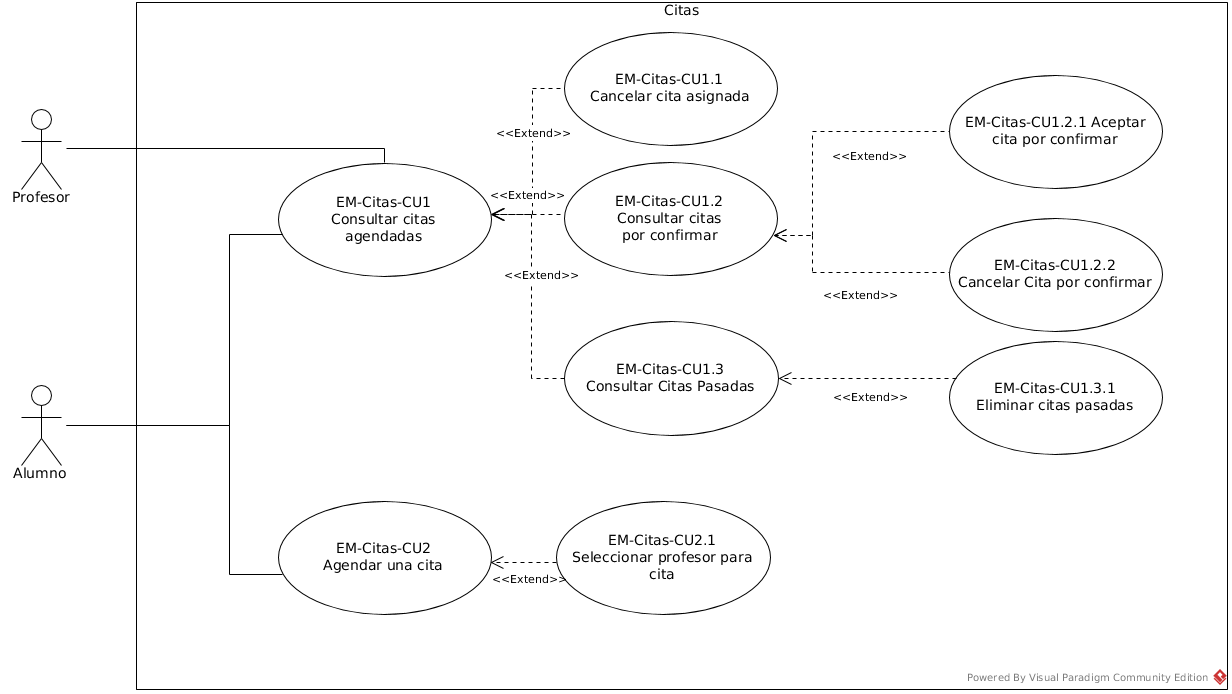
\includegraphics[width=1\textwidth]{images/casos/cita}
	\caption{Diagrama de casos de uso ESCOMobile: Citas.}
\end{figure}


%%%%%%%%%%%%%%%%%%%%%%%%%%%%%%%%%%%%%%%%%%%%%%%%%%%%%%%%%%%%%%%%%%%%%%%%%%%%%%%%%%%%%%%%%%%%%%%%%%%%%%%%%%%%%%%
%											MÓDULO DE BOLSAWEB
%%%%%%%%%%%%%%%%%%%%%%%%%%%%%%%%%%%%%%%%%%%%%%%%%%%%%%%%%%%%%%%%%%%%%%%%%%%%%%%%%%%%%%%%%%%%%%%%%%%%%%%%%%%%%%%


\section{Módulo de BolsaWeb}

\noindent
Este módulo presenta todo el proceso que se realiza detrás de la bolsa de trabajo y las ofertas 
propuestas que se enuentran disponibles para consulta en ESCOMobile. Aquí se describen los diferentes
procesos como el registro, consulta, edición y eliminación de empresas y ofertas de trabajo que
éstan proporcionan, así como la publicación de la información en distintos medios en la red.
El módulo se complementa con AlumnoBolsa para formar un gran módulo llamado ESCOMobile Bolsa,
se compone de 10 casos de uso, que se enlistan ahora. 

\begin{requisitos}{EM-BolsaWeb-CU1}
	\RFitem{Nombre}{Gestionar Ofertas de Trabajo.}
	\RFitem{Actores}{Encargado dpto. de Extensión y servisios eductativos.}
\end{requisitos}

\begin{requisitos}{EM-BolsaWeb-CU1.1}
	\RFitem{Nombre}{Añadir Oferta de Trabajo.}
	\RFitem{Actores}{Encargado dpto. de Extensión y servisios eductativos.}
\end{requisitos}

\begin{requisitos}{EM-BolsaWeb-CU1.2}
	\RFitem{Nombre}{Editar Oferta de Trabajo.}
	\RFitem{Actores}{Encargado dpto. de Extensión y servisios eductativos.}
\end{requisitos}

\begin{requisitos}{EM-BolsaWeb-CU1.3}
	\RFitem{Nombre}{Eliminar Oferta de Trabajo.}
	\RFitem{Actores}{Encargado dpto. de Extensión y servisios eductativos.}
\end{requisitos}

\begin{requisitos}{EM-BolsaWeb-CU2}
	\RFitem{Nombre}{Consutlar Estadísticas de la Oferta.}
	\RFitem{Actores}{Encargado dpto. de Extensión y servisios eductativos.}
\end{requisitos}

\begin{requisitos}{EM-BolsaWeb-CU3}
	\RFitem{Nombre}{Publicar Boletín de Ofertas de Trabajo.}
	\RFitem{Actores}{Encargado dpto. de Extensión y servisios eductativos.}
\end{requisitos}

\begin{requisitos}{EM-BolsaWeb-CU4}
	\RFitem{Nombre}{Gestionar Empresas.}
	\RFitem{Actores}{Encargado dpto. de Extensión y servisios eductativos.}
\end{requisitos}

\begin{requisitos}{EM-BolsaWeb-CU4.1}
	\RFitem{Nombre}{Añadir Nueva Empresa.}
	\RFitem{Actores}{Encargado dpto. de Extensión y servisios eductativos.}
\end{requisitos}

\begin{requisitos}{EM-BolsaWeb-CU4.2}
	\RFitem{Nombre}{Eliminar Empresa.}
	\RFitem{Actores}{Encargado dpto. de Extensión y servisios eductativos.}
\end{requisitos}

\begin{requisitos}{EM-BolsaWeb-CU4.3}
	\RFitem{Nombre}{Editar Información de la Empresa.}
	\RFitem{Actores}{Encargado dpto. de Extensión y servisios eductativos.}
\end{requisitos}

\noindent
A continuación se muestra el diagrama de casos de uso correspondiente a este módulo.

\pagebreak
\begin{figure}[htbp!]
	\centering
	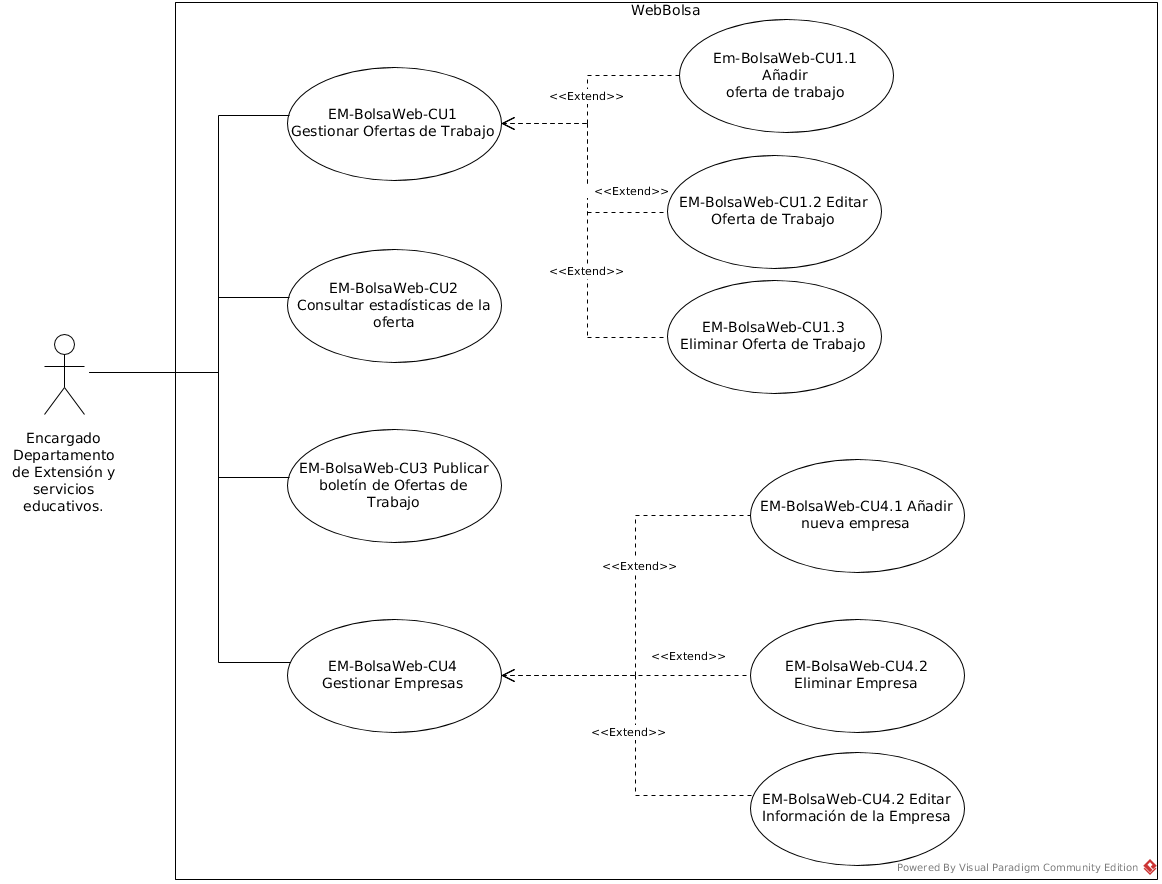
\includegraphics[width=1\textwidth]{images/casos/WebBolsa}
	\caption{Diagrama de casos de uso ESCOMobile: BolsaWeb.}
\end{figure}


%%%%%%%%%%%%%%%%%%%%%%%%%%%%%%%%%%%%%%%%%%%%%%%%%%%%%%%%%%%%%%%%%%%%%%%%%%%%%%%%%%%%%%%%%%%%%%%%%%%%%%%%%%%%%%%
%													ESCOMOBILE
%%%%%%%%%%%%%%%%%%%%%%%%%%%%%%%%%%%%%%%%%%%%%%%%%%%%%%%%%%%%%%%%%%%%%%%%%%%%%%%%%%%%%%%%%%%%%%%%%%%%%%%%%%%%%%%


\section{Integración de ESCOMobile}

\noindent
Finalmente, se muestra el diagrama general de casos de uso, que engloba todos los módulos antes descritos,
la forma en que se conectan y se comunican unos con otros, así como con la interacción de los cuatro actores 
contemplados en ESCOMobile (Alumno, Profesor, Invitado y Encargado dpto. de Extensión y servisios eductativos).
Es así como se forma la aplicación ESCOMobile, compuesta por ocho módulos y un total de cuarenta y cinco
casos de uso. 

\pagebreak
\begin{figure}[htbp!]
	\centering
	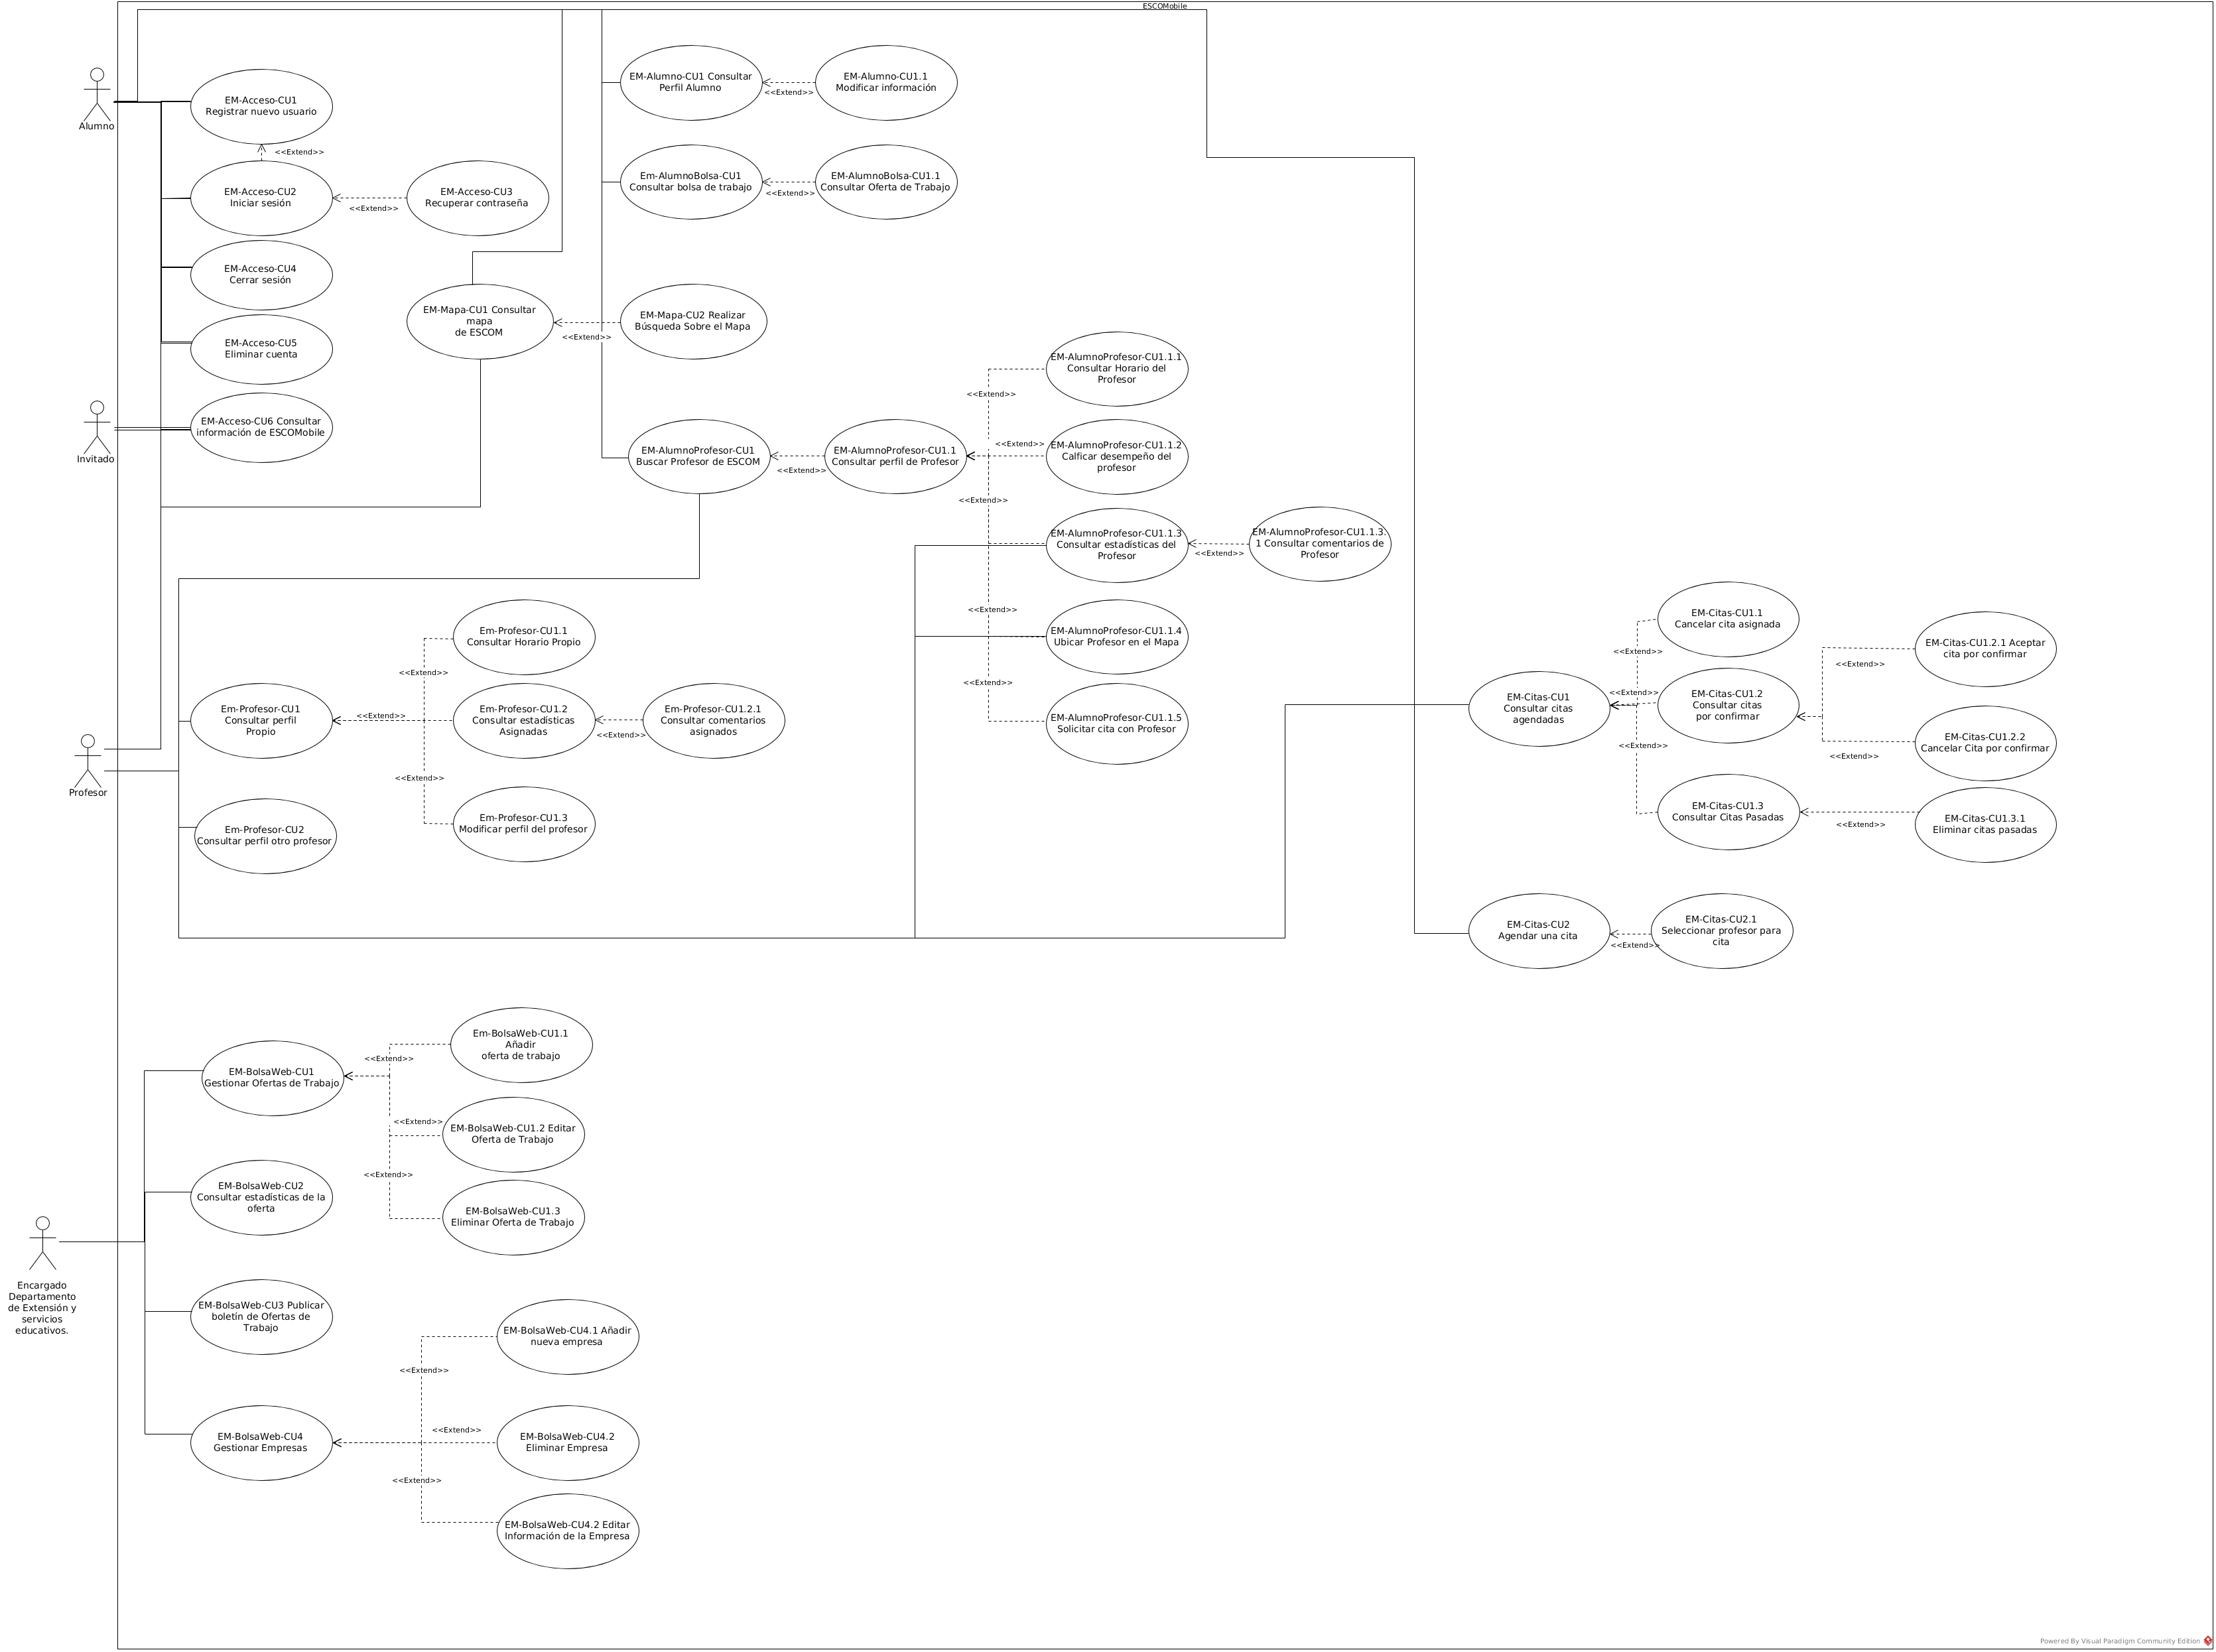
\includegraphics[width=1\textwidth]{images/casos/general}
	\caption{Diagrama general de casos de uso ESCOMobile.}
\end{figure}